% This is samplepaper.tex, a sample chapter demonstrating the
% LLNCS macro package for Springer Computer Science proceedings;
% Version 2.20 of 2017/10/04
%
\documentclass[runningheads]{llncs}
% UTF-8 encoding and Norwegian letters æ, ø, å, etc. accepted
\usepackage[utf8]{inputenc}
\usepackage[T1]{fontenc}

\usepackage{graphicx}
\usepackage{listings}
\usepackage{xcolor}
\usepackage{AMMALanguages}

% Used for displaying a sample figure. If possible, figure files should
% be included in EPS format.

\usepackage{hyperref}
\definecolor{medium-blue}{rgb}{0,0,1}
\hypersetup{colorlinks, filecolor={medium-blue}, linkcolor={medium-blue}, urlcolor={medium-blue}}
% If you use the hyperref package, please uncomment the following line
% to display URLs in blue roman font according to Springer's eBook style:
\renewcommand\UrlFont{\color{blue}\rmfamily}

% New command for prettifying C++ 
% Usage: \cpp\ (last backslash needed for space after C++)
\newcommand{\cpp}{C\nolinebreak\hspace{-.05em}\raisebox{.4ex}{\tiny\bf +}\nolinebreak\hspace{-.10em}\raisebox{.4ex}{\tiny\bf +}}

% New command for prettifying C# 
% Usage: \csharp\ (last backslash needed for space after C#)
\newcommand{\csharp}{%
  {\settoheight{\dimen0}{C}C\kern-.05em \resizebox{!}{\dimen0}{\raisebox{\depth}{\#}}}}

% Custom hyphenations
\hyphenation{meta-methods}


% TODO: Hyperlinks not working..?!


\begin{document}
%
\title{CommonLang: a DSL for defining robot tasks} %\thanks{Supported by organization x.}}
%
%\titlerunning{Abbreviated paper title}
% If the paper title is too long for the running head, you can set
% an abbreviated paper title here
%
\author{Adrian Rutle\inst{1}\hspace{-3pt}~\and
Jonas Backer \inst{1}\hspace{-3pt}~\and
Kolbein Fold{{\o}}y\inst{1}\hspace{-3pt}~\and
Robin T. Bye\inst{2}
}
%
\authorrunning{A. Rutle et al.}

\institute{Western Norway University of Applied Sciences, Bergen, Norway
\email{\{aru,149906,149909\}@hvl.no}\\ \and
Cyber-Physical Systems Laboratory, \\
%Department of ICT and Natural Sciences, \\
%Faculty of Information Technology and Electrical Engineering, NTNU\\
NTNU---Norwegian University of Science and Technology, Ålesund, Norway\\
%Postboks 1517, NO-6025 Ålesund, Norway\\
\email{robin.t.bye@ntnu.no}}
%
\maketitle              % typeset the header of the contribution
%
\begin{abstract}
Robots are becoming more and more complex and heterogeneous; their abilities and domains of usage are increasing exponentially.
Programming these robots requires special skills and usually does not follow standard software engineering methodologies.
Adhering to model-driven software engineering principles, definition of robot behaviour is abstracted and represented in models while robot-specific code is generated from these models using code generation.
With a robot modelling framework, we can work on a higher abstraction level making the task of programming complex heterogeneous robots more efficient.
In this paper, we present such a modelling framework and evaluate its flexibility by extending it with wireless communication functionalities.

\keywords{Robot programming  \and Robot modelling framework \and Model-driven software engineering \and Robot communication protocol.}
\end{abstract}

\section{Introduction}
Robots come in a variety of sizes and shapes and with different purposes and abilities.
In today’s society robots have revolutionized the efficiency and productivity in many fields. 
The use of robots in the field of manufacturing cars has increased the capacity and quality of the cars, in addition to protecting workers from performing extremely dangerous tasks.
In agriculture, drones are being used to analyze soil and plant seeds and  choosing the best moment to harvest. 
Whether robots are used for bomb disposal or vacuum cleaning, their operation depends on both their hardware and the software they are running \cite{mazur16}.

Current robot programming frameworks require both a steep learning curve and specific hardware and software environments.
A large number of robotic software exist but interoperation across robots is difficult, with dependencies on specific hardware or software platforms that are hard-wired into the robot code \cite{Dhouib2012robotml,Dragule}.
Addressing recent challenges in robotics~\cite{Yang2018challenge} has led to various conference and workshop series focusing on robotics software and design~\cite{RoboticsSummit2018}.
Specifically, using model-driven software engineering  (MDSE) methodologies and technologies to raise the abstraction level of robotic software development, enable simulation and verification, and tackle complexity challenges, are common research goals at events such as MORSE, SIMPAR, ICRA, ROSE, etc.

In this paper, we present a prototype framework \textit{CommonLang} (CoL) which uses MDSE-techniques~\cite{Brambilla2017,brugali2015model} to
abstract away from underlying technologies and create executable code for various different robot platforms using code generation \cite{gya17}.
The framework comes with a text-based domain-specific language (DSL) that enables users to write scripts through abstracted \textit{metamethods}; i.e., function abstractions providing a higher-level language.

Given a number of heterogeneous robots, each with its own programming language, the main feature of CoL is its ability to parse a common set of robot instructions into multiple tailor-made scripts to yield identical behaviour for the robots.  
The layout of the output scripts is dependent on XML configuration files that contain the implementation of the metamethods and specify what language they should be parsed to (e.g., C, Python, Java, etc.).
In this paper, we demonstrate behavioural programming of two robots that use C/\cpp\ and Python, respectively, as well as providing an evaluation of CoL's ability to avoid increased complexity---keeping usability and ease of access at an acceptable level---when adding WiFi communication functionality by utilizing metamethods.




\section{CommonLang}


\begin{figure}[b]
	\centering
    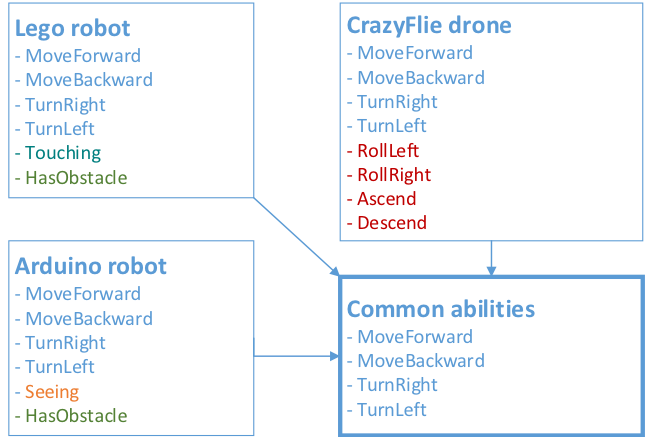
\includegraphics[scale=0.65]{./images/commonlang.png}
    \caption{Example of common abilities in different robot platforms.}
    \label{fig:commonlang}
\end{figure}


CommonLang (CoL)---which was first described in \cite{gya17}---is a DSL created specifically for writing code for a set of various robots using different programming languages. 
It is an imperative and structured language, and in many ways similar to Java,
which is one of the languages CoL can be parsed to.
CoL includes various control flow constructs found in most other programming languages, e.g., \texttt{for}, \texttt{if}, and \texttt{while} statements.

The aim of CoL is to enable reusable behavior for different robots with similar abilities. 
To accomplish this goal, a textual DSL was defined using Xtext in Eclipse~\cite{xtext}.
The solution builds on the concept of metamethods that declare the common abilities of target systems for a behavioral script. 
Fig.~\ref{fig:commonlang} illustrates how the 
functionality of three different robot platforms can be used to create a common set
of abilities, consisting of the metamethods that can be used in scripts targeted to these platforms. 
%REVIEW
These commonalities are not enforced, meaning that robots which do not naturally exhibit common functionalities will not be sharing behavior.
However, in the CoL script it is possible to use metamethods that are not present in all target platforms.
The invocation of these will be ignored on unsupported platforms.
In this way, a script can define tasks for a heterogeneous environment of interacting robots.





\subsection{Defining behavior with CoL scripts}



Defining behavior in CoL consists of two steps: writing a CoL script and listing the collection of metamethods. 
The script is declared by the script keyword, the script name, then the target keyword, and finally the platforms to be targeted (see Fig.~\ref{fig:commonlang-script}).
The script is written in a file with the extension name \texttt{.commonlang} and consists of two main blocks. 
The first part contains the \texttt{script} definition, name of the script (\texttt{MyScript}), and a set of what robots the script will be generated for (\texttt{LegoMindstormsEV3} and \texttt{ArduinoShieldBot}), in the form of configuration file names for each robot.
Target platforms must include a specific configuration for each platform as many robot platforms allow the hardware to be configured differently as needed. 
Scripts may consist of variables, metamethod invocations, and some common control statements such as \texttt{if}, \texttt{else}, and \texttt{while}.
The program code will be written inside a method called \texttt{loop} contained in the script block, and consists of user methods and metamethods. 
The output code, here parsed to Arduino (C/\cpp) and Python, will continuously iterate this method, hence it does not allow for storing states, like integers and booleans. 

\begin{figure}[t]
	\centering
	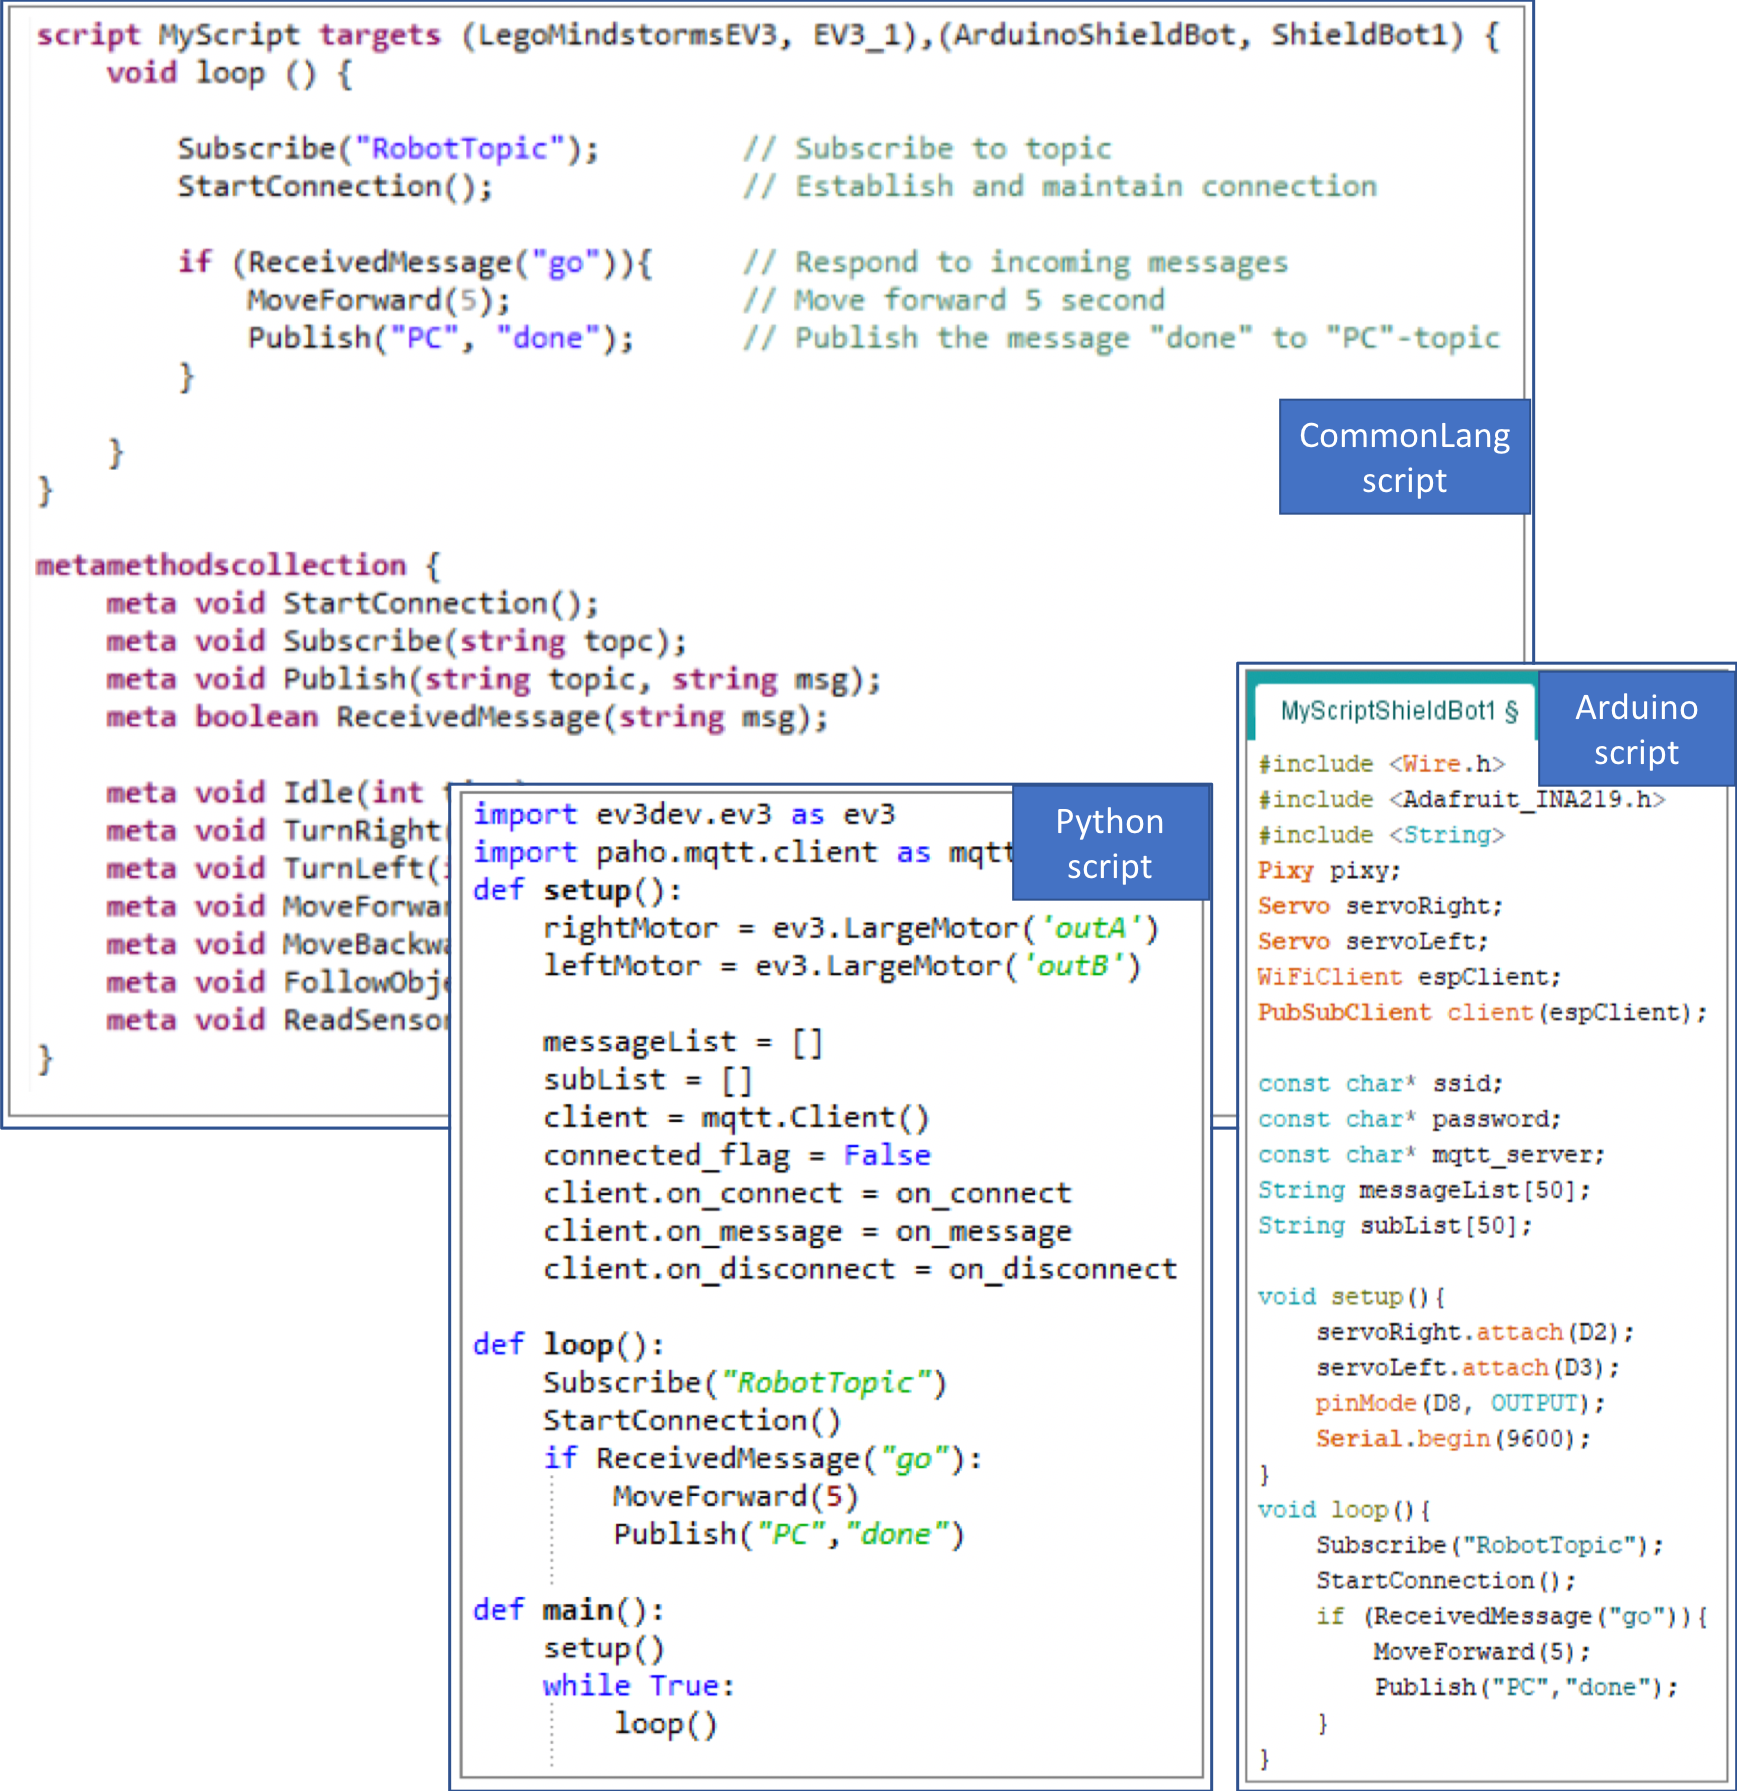
\includegraphics[width=\linewidth]{images/commonlang-short.png}
	\caption{Sample CommonLang program with code-generation to Python and C}
	\label{fig:commonlang-script}
    \vspace{-6mm}
\end{figure}

The second block is called \texttt{metamethodcollection}, which is a set of predefined methods that every robot with a different programming language is able to run and has its own implementation of. 
Each metamethod declaration consists of the reserved keyword \texttt{meta}, followed by a return type, name and its corresponding parameters. 
For example, the metamethod \texttt{MoveForward} may for some robots make two of the wheels spin forward, whereas for other robots may make four wheels spin at different speeds. 
Some robots may even be flying, meaning they will have rotors spinning in different directions to be able to fly forward. 

For CoL to generate code for a robot's native language, we need to declare two XML files (see Fig.~\ref{fig:commonlang-xml}). 
The first XML file is generic for all robots of its kind and contains various types of data, such as the file format for the language files (e.g., \texttt{.py} or \texttt{.c} indicating Python or C files, respectively), global variables, declarations and method calls for the setup method of the final script. 
It also contains which metamethods the robot can execute. 
In this XML file, the metamethods have a simple code segment, either calling its corresponding method from the other XML file where it is implemented, or returning a value from global variables or forwarding the return value from the method it is calling~\cite{gya17}.
\begin{figure}[t]
	\centering
	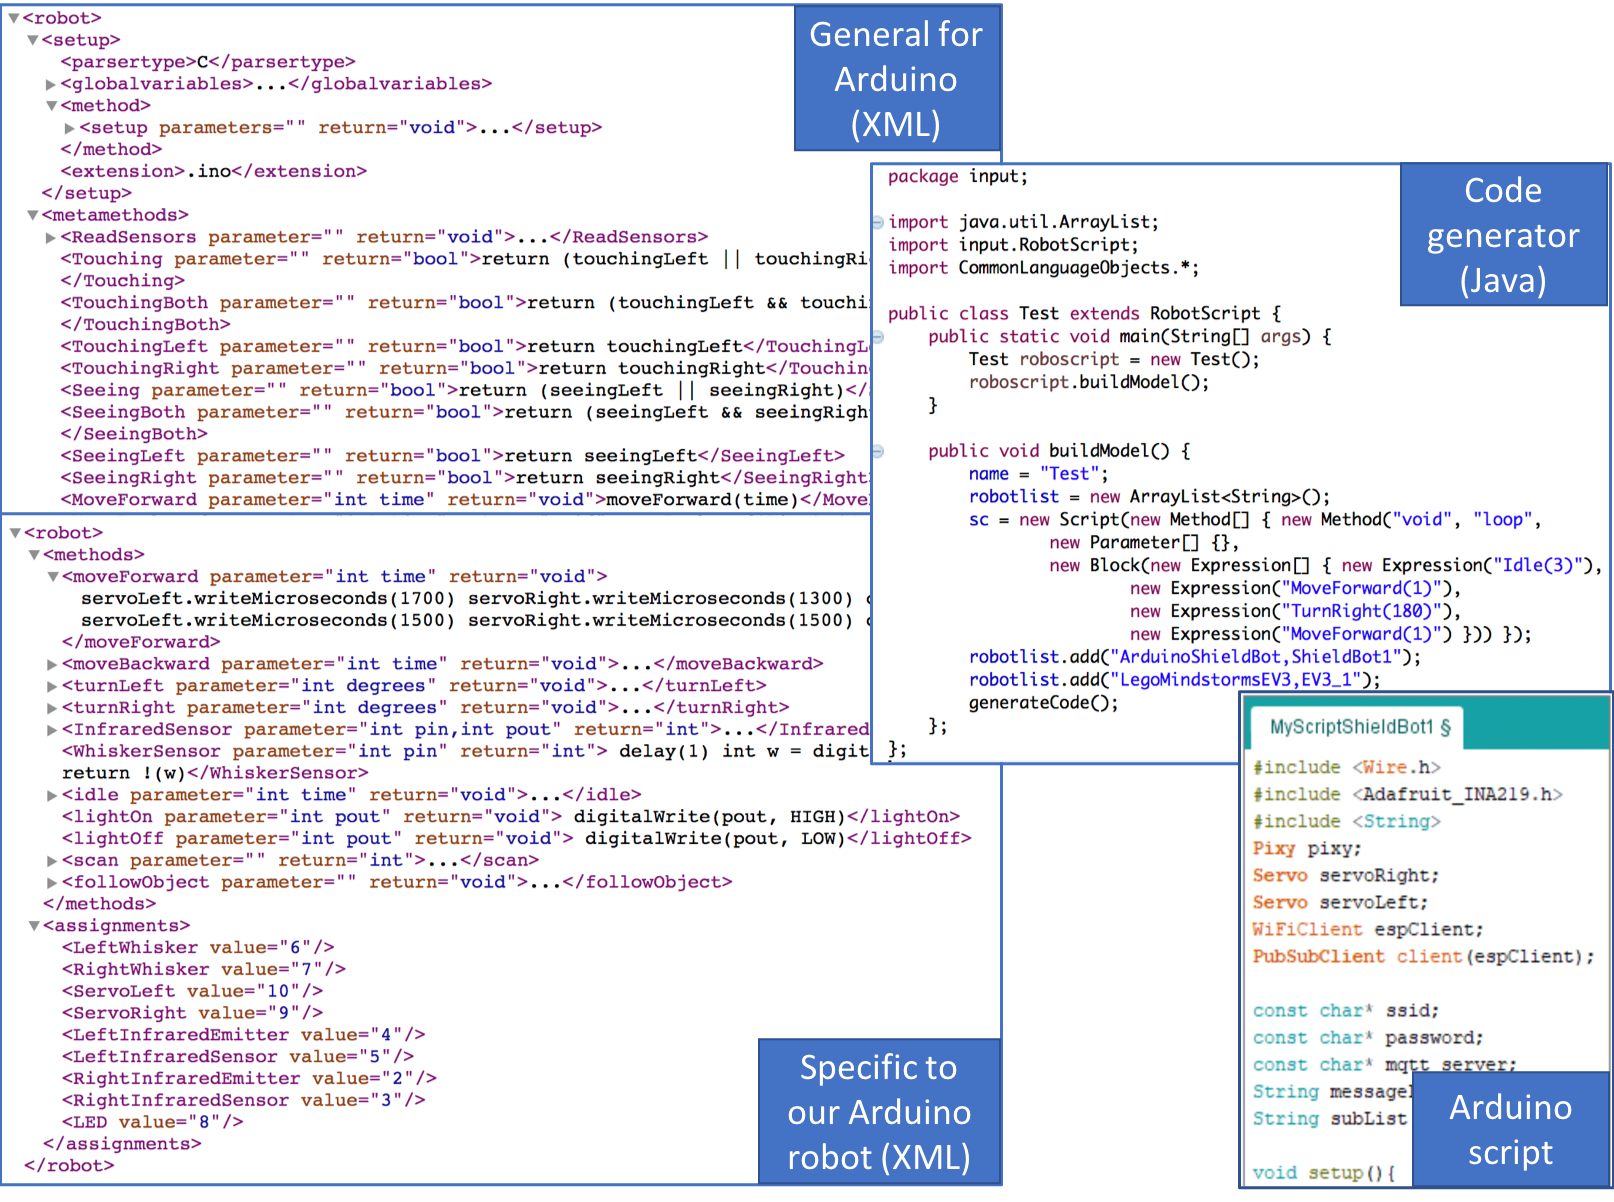
\includegraphics[width=\linewidth]{images/structure-xml-2.png}
	\caption{XML configuration files}
	\label{fig:commonlang-xml}
    \vspace{-3mm}
\end{figure}


The other XML file is specific for the robot configuration and contains the implementation of the methods in the robots’ own language, for instance, setting a motor to run for the duration specified in the parameters or reading the value of a digital pin and returning it. 
These methods with their implementations are then automatically added without changes to the final output script which is already in the target language. 
Additionally, this XML file contains a tag called \texttt{assignments} for setting up robot sensors to the right pin values, since this configuration is robot-dependent.

\subsection{Code generation from CoL scripts}

As mentioned, the CoL grammar is defined in Xtext~\cite{xtext}.
The details of Xtext and how it works is out of the scope of this paper, but in short, Xtext facilitates the definition of DSLs using a powerful grammar language and as a result we can get a full DSL-infrastructure, including parser, linker, typechecker, compiler as well as a language editor with syntax-highlighting in Eclipse.
CoL relies on code-generation functionalities provided by Xtext.
These functionalities are defined as templates in the language Xtend---a flexible and expressive dialect of Java which compiles into readable Java 8 compatible source code.
To understand how this code-generation step works, we include an excerpt of the CoL grammar in Listing~\ref{lst:grammar}.
Xtend creates a Java class for each language construct in the grammar, e.g. \texttt{Script.java}, \texttt{MetaMethods.java}, \texttt{Block.java}, etc.
In addition to these classes, we have implemented a class \texttt{BotMethods.java} which parses the two XML files for each robot in the \texttt{targets} block.
Following the Xtext methodology, we have also implemented a customized code-generator class for each target language; in this case one for \texttt{Python} and one for \texttt{C}.

Once a valid CoL script (according to the grammar) is saved, all these classes gets instantiated automatically by the Xtext language-infrastructure.
In addition, a code generator (which is a simple Java program as shown in Fig.~\ref{fig:commonlang-xml}) will be generated automatically for each CoL script.
Running this Java program will create the final robot scripts for the target platforms.

\begin{lstlisting}[breaklines,style=AMMA,language=Xtext,mathescape,rulesepcolor=\color{black},caption=\small{Grammar of CommonLang} ,captionpos=t,label={lst:grammar},numbers=left]
  grammar org.xtext.Commonlang with org.eclipse.xtext.common.Terminals

  generate commonlang "http://www.xtext.org/Commonlang"

  CLfile:
	scripts+=(Script)*
	mets=MetaMethods;
  Script:
	'script' name=CAPITALFIRST 'targets' '(' robottypes+=(LOWERFIRST | CAPITALFIRST) ',' robotconfigs+=(LOWERFIRST |
	CAPITALFIRST) ')' (',' '(' robottypes+=(LOWERFIRST | CAPITALFIRST) ',' robotconfigs+=(LOWERFIRST | CAPITALFIRST)
	')')* '{'(methods+=UserMethod*)'}';
  MetaMethods:
	{MetaMethods} 'metamethodscollection' '{'(methods+=MetaMethod)*'}';
  Block:
	{Block} '{' ((exs+=SimpleExpression ';' | exs+=StructureExpression))* '}';
  SimpleExpression:
	Crement | Call | Assignment | Return;
  StructureExpression:
	Block | If | For | While;
  Expression:
	SimpleExpression | StructureExpression;
//...
  Method:
	(UserMethod | MetaMethod);
  MetaMethod:
	'meta' type=Methodtype name=CAPITALFIRST '(' parameters+=Declaration? (','+ parameters+=Declaration)* ')' ';';
  UserMethod:
	type=Methodtype name=LOWERFIRST '(' parameters+=Declaration? (','+ parameters+=Declaration)* ')' bl=Block;
//...
\end{lstlisting}

% The CoL script is then parsed into the a code generator which is a Java program.
% This program uses functionalities from a class called \texttt{RobotScript} in order to generate the specific code for the robots defined as parameters to the \texttt{target} keyword.
% The two XML files are used in this step to configure the final script.

Using the standard Xtext methodology, code-generation is divided into two steps.
Firstly, an object model will be created for the parsed CoL script, then, target scripts in the native languages of the robots will be created using the customized code-generators.
The complexity of these code generation steps depends on the complexity of the CoL script and the number of robot kinds which are defined in the \texttt{targets} block.
These steps are hidden from the CoL script and metamethod developers.

Extending CoL with support for generating code to new target platforms require some knowledge of Java and Xtext. 
This consists of implementing a Java class for each new target language (however, C and Python covered all the robots which we have had in hand, e.g. Arduino robot, Lego Mindstorm, CrazyFlie mini-drones and Land-rovers with Raspberry PI 3).
In the envisioned scenario, this activity is hidden from CoL script developers and delegated to DSL-infrastructure experts.

Configuring and developing metamethods are done in the XML files. 
Our optimal goal is to ship the DSL with a number of most-used metamethods for various commonly available robots.
However, we see this activity as a community effort and envisage that the future of the DSL will be depending on the availability of this infrastructure.
We have currently not defined any scheme or convention for the definition of these metamethods due to their simplicity, however, in future work we plan to define a guideline and a metamodel in form of an XML Schema Definition (XSD) for the configuration XML files.

\section{Extension with Wireless Communication}

In order to evaluate the DSL, we have extended its functionality by adding features for WiFi communication using Message Queuing Telemetry Transport (MQTT) \cite{MQTT}  as a sample communication protocol. 
This functionality is not hard-coded and can be replaced by other protocols if needed. 

MQTT is a lightweight messaging protocol that allows the robots to subscribe to topics. 
They can also publish messages to the topics, so that clients subscribed to a particular topic will receive the messages. 
A broker is required for this setup to work. 
It keeps track of available topics and clients connected to the server, forwarding incoming messages to all the clients subscribing the respective topics.
For a client to subscribe to a topic it needs only to know the IP address of the broker.
We have used the Eclipse Mosquitto \cite{MOSQUITTO} implementation of MQTT, which grants the ability to set up a broker and enter commands such as subscribing and publishing messages to desired topics into the command prompt window.


An important decision had to be made regarding whether the communication should be integrated as part of the CoL grammar or as additional metamethods through the XML files. 
Editing the grammar of the language results in fewer unnecessary lines of code in the XML files.
%Minimizing the size of the program code becomes especially important considering some robots may have a very limited program memory onboard. 
However, modifying the CoL grammar is more complex than making metamethods for it: 
the DSL is designed for handling metamethods specified in the robots’ XML files.
It creates an environment for general purpose robot programming which could be compromised by adding grammar specifically for MQTT communication since with further development of the language other communication protocols may be desirable. 
By refraining from doing grammatical adjustments, it becomes quite manageable to add or edit already existing metamethods for communication.

A crucial part of integrating communication through metamethods is making the code intuitive and user-friendly, and at the same time not limiting what the end user is able to do. 
Various approaches to how the syntax and methods should look like have been considered. 
One of the approaches was to let the end user create a  method surrounding a selection of metamethods. 
This user method would then be connected to a message string through a metamethod called \texttt{OnMessage}. 
This is how it would look like:


\begin{lstlisting}[breaklines,style=AMMA,language=java,mathescape,rulesepcolor=\color{black},caption=\small{OnMessage metamethod} ,captionpos=t,label={lst:T},numbers=left]
OnMessage("go", forwardAndLightsOn);

void forwardAndLightsOn() {
	MoveForward();
	LightsOn();	
}
\end{lstlisting}




This approach would result in more code to write. 
It would also require a change in the language’s grammar, allowing it to take a method as a parameter. 
After considering variations of similar syntax, we settled on utilizing the simplicity of metamethods combined with \texttt{if} statements, which are already part of the Commonlang grammar.
The metamethod is called \texttt{ReceiveMessage} and takes a single string parameter, returning a boolean value. Here is an example:


\begin{lstlisting}[breaklines,style=AMMA,language=java,mathescape,rulesepcolor=\color{black},caption=\small{ReceiveMessage metamethod} ,captionpos=t,label={lst:T2},numbers=left]
if (ReceivedMessage("go")) {
	MoveForward();
	LightsOn();
}
\end{lstlisting}


The method is checking whether the robot has received a specific message. 
When the robots receive messages, the method triggers a callback called \texttt{on\_message} that will put the messages in a list. 
This is because the callback method is hardcoded in the XML files and cannot be dynamically changed. 
Instead, this \texttt{ReceivedMessage} method was created to scan through the message list to check for the string from its parameter. 
If it finds it, a single instance of the message will be removed from the list and it will return true; otherwise false.

%TODO Do we need all these? A short version should be enough here! NEI
% In addition to the \texttt{ReceivedMessage}, there are three other important metamethods that is implemented as part of the communication in Commonlang. 
% These are called \texttt{StartConnection}, \texttt{Publish} and \texttt{Subscribe}. 
% \texttt{StartConnection} is a method that takes no parameters and has no return value. 
% It has two important features: 
% The first is to establish and maintain a connection with the broker, and the second is running a MQTT-specific method that is called \texttt{client.loop}. 
% The \texttt{client.loop} method needs to be continuously run as it allows the client to process the incoming messages. 
% It was discussed whether the method should accept parameters allowing the end user to choose, for instance the brokers IP address. 
% To keep the Commonlang code as clean and simple as possible, we concluded that this can rather be changed in the XML. 
% \texttt{StartConnection} should be in the top of the main loop method of the program as a connection is required for the rest of the connection methods to be functional. 
% To be able to publish messages to a topic of one’s choice, the \texttt{Publish} method will take two parameters: the topic name and the message content. 
% The \texttt{Subscribe} method is taking a string parameter with the name of the topic one want to subscribe to. 
% However, once the Subscribe method has been run, the MQTT method \texttt{client.subscribe} has not been run yet. 
% Initially, the callback \texttt{on\_connect}, which is called when the connection is established, would run the \texttt{client.subscribe} for a predefined/hardcoded topic. 
% To be able to dynamically choose the topic via Commonlang, a list of topics was created. 
% The Subscribe method will put the topic name into this list, and the \texttt{on\_connect} callback will run client.subscribe on every element of the list. 
% As it can take about a second to establish a connection to the broker, it is not necessary to write the Subscribe methods in the CoL before \texttt{StartConnection}, although it is recommended.


% \section{Case Study}

% In order to evaluate the DSL, a case-study was performed using test subjects to implement the behaviour of two robots using a single CoL script.
% The case study is an implementation of the ``Red Light Game'' which consists of a leader and a group of players. 
% The goal is to be the first player of the group to reach the leader. 
% However, the group may only advance towards the leader when he/she is not looking. 
% If the leader catches a player moving when facing them, the player in question loses and will have to start from the beginning again. 

% Two robots were used during the case study: (i) a Lego Mindstorm EV3 robot programmed in Python running "ev3dev" \cite{EV3DEV} with the "Brickman" software \cite{BRICKMAN}, and 
% (ii) a custom-made Arduino-based robot programmed in C/\cpp\ with a Parallax robot shield~\cite{parallax}.
% The Arduino robot at disposal for the case study is already equipped with an original Arduino board. 
% The board itself does not have hardware that allows it to send and receive data wirelessly. 
% An external shield/board is required to give the board the ability to connect to other devices, or, the Arduino board on the robot can be replaced with the Wemos D1 WiFi board, which was the chosen solution. 

% The Arduino robot is equipped with multiple sensors and two continuous servos. 
% Since the Arduino robot does not have a gyroscope, getting it to turn an exact number of degrees turned out to be challenging, since this operation depends on surface friction, battery voltage, and accuracy of the servos. 
% However, the colour-tracking Pixy camera mounted on top of the robot solves most of these issues when it is most critical, that is, when the robot is facing a certain direction~\cite{parallax}. 

% The Pixy camera is calibrated on a computer to track certain colours, and is used to turn to a specific player in the Red Light Game and check for movement of that player. 
% It measures the width of the tracked object and looks for a pixel change in this value beyond a certain threshold. 
% If movement is confirmed it publishes a “loss” message to the one in question and this player must start over from the startline \cite{rowe15}. 
% The Arduino robot also has a couple of whiskers used to determine when it has bumped into something. 
% %This could be used if it is going to take the place of a player and needs to identify then it has won.

% In the game, the Arduino robot has to send messages to the other robots playing about stopping and losing. It subscribes only to the message that starts the game sent from the computer.
% %As stated previously the Wemos board runs MQTT as its communication protocol. 
% %It does this by importing and declaring a \texttt{PubSubClient}. 
% %This client then looks for specifically named variables and methods to be set and called at specific times. 
% The Arduino robot acts as the leader, whereas the EV3 robot is a player. The robots are positioned two meters apart facing each other and the game starts when the Arduino gets the go ahead from the PC. The Arduino robot then turns 180 degrees, which is noticed by the EV3. The EV3 starts moving slowly towards the Arduino robot, until it gets a “red light” message from the Arduino. The message is sent once the Arduino robot is midway turning back towards the EV3. The EV3 should now be at a standstill and the Pixy camera will start looking for significant movement of the reflector on the EV3. If the Pixy does not sense a movement above a threshold the Arduino robot will turn back again, and the EV3’s sonic sensor will tell it to move.  
% If the Pixy camera notices the EV3 moving when it should not, it will send it a ``loss'' message and the EV3 will move back to start.    
% This continues until the EV3 has reached the Arduino robot with its touch sensor.

% % \section{Evaluation}

% % %TODO Rewrite and shorten this paragraph, too much BS!
% % Testing was performed both during and after completion of the case study. 
% % Artifact testing was carried out where possible, and functional testing otherwise. 
% % In addition, an evaluation of functionality and ease of access was performed as the DSL was made to cater to users of less understanding of the concepts of programming robots. 
% % The case study falls under two categories of evaluation methods as it is both qualitative---if we consider it as subjective interviews---and design science oriented as a human to computer artefact.
% % %As for ex-post artifact evaluation of the project there are several interpretations of how to evaluate such artifacts as our expansion package to CoL. 

% % The test subjects were asked to make a simple script containing all metamethods used for communication and a single metamethod from the core with some logic. The commonlang robotscript would make the robot start a connection to the broker, tell another robot to move forward and check for an incoming message to move forward. They were given a simplified explanation of what the metamethods did as well as how the MQTT communication protocol worked.

% Through the case studies we found that the test subjects could write scripts in CoL language with the communication extension with relative ease. 
% The subjects found the setup and syntax of the language familiar, and the use of metamethods similar to using a package. 
% The scripts they made would run fine on the robots and fulfilled the requirements requested. 
% They also found most of the naming of metamethods made sense. Only one problem arose, the metamethod \texttt{boolean ReceivedMessage(string msg)} returns true if the robot has received the message parameter. 
% The subjects expected it to also contain a topic parameter as to know where the message came from. 
% If one would like to identify where the message came from, one would have to use different messages depending on who sent it. 
% The reason for this design choice was to be able to react to a message independent of where it came from without having to check if that message was received from each of the robots.


% %TODO Should some of this be moved to future work?
% %ARU: Since this is an evaluation section, perhaps we should keep some claims here. Perhaps repeat some of these later?
% From our evaluation, the script fulfilled the requirements of the assignment, however there are still improvement potential both when related to the DSL, metamethod performance, and ease of access. The wireless communication extension could also have been made available as a module package, making it even more convenient if a change in communication protocol is needed.       

\section{Related Work}

Robots can be programmed in different ways: from writing robot-specific code directly to using frameworks with varying functionality. 
Some of these frameworks, such as Papyrus-RT \cite{PAPYRUS-RT} and RobotML~\cite{Dhouib2012robotml}, utilize MDSE techniques~\cite{Brambilla2017,brugali2015model} to deal with software complexity.
Others, such as the Robot Operating System (ROS)~\cite{ROS} and RoboDK~\cite{RoboDK}, use programming frameworks which are tailored for specific kinds of robots.
Below we shortly introduce these frameworks, keeping in mind that the main distinctive characteristic of CoL is its support for writing behavior for a heterogeneous environment of various kinds of robots.
 
ROS is an open source project consisting of a collection of tools, libraries and conventions that aims to simplify programming robust and complex behaviour of robots of all shapes and sizes across a wide variety of platforms, whereas
Papyrus-RT is another framework for real-time programming of robots which generates \cpp\ code from models defined in the UML-RT modeling language.
RobotML is a DSL that aims at solving several central problems with robot programming today~\cite{Dhouib2012robotml} such as costs and difficulty of development and reusability issues because of low level details being hard-wired into the code at early stages in the development. 
Interaction modelling~\cite{cornelius2017model}, Deep modeling~\cite{atkinson2014towards}, and Multi-robot systems~\cite{di2014family} also use DSLs for modeling robotic software but they do not have the same maturity as RobotML and Papyrus-RT.
The robot instructions written in these languages can be simulated and visualized in 3D as well as exported to the native languages of each of the robots.
Unfortunately, RoboDK currently only supports industrial robots.

\section{Conclusion and Future Work} 

%The target users of CoL might be laypersons wanting to program robots without needing to know the inner workings of a specific script. 
%The language caters well to professionals or hobbyists wanting to program similar robots that interpret different languages. 
% Lower level metamethods give great customizability, but also increases the overall difficulty. 
% Higher level metamethods are specific and somewhat limiting but offers a great amount of functionality compared to how much work and understanding is required by the CoL user~\cite{gya17}.

%TODO Needed?
We have presented CoL, a DSL for robot task specification which enables compilation of tasks to heterogeneous robot platforms.
%Programming of robots with similar functionality can be time-consuming even if the robots share traits. 
With CoL, one can do the time-consuming work of writing functions and setup once, then use these functions to define tasks for robot teams. 
The functions are developed as metamethods which extend what the users can express with CoL scripts. 
%Making these general abstract functions will later allow for faster and easier programming.
Since one could make any kind of metamethods, the functionality can vary greatly from a simpler move-forward function to highly abstract functions such as ``water field'' or ``defuse bomb.'' 
The defined functionality is contained within XML configuration files that are included in CoL scripts. 
This means one could make these robot-specific files beforehand and make documentation for them so that the CoL scripts can be written by less technical domain-experts to define heterogeneous robot behavior in various domains.
These domains could be anything as long as the tasks in the CoL script can be achieved by robots for which the appropriate metamethods are implemented.
The usability and extendability of CoL was demonstrated by adding support for wireless communication.
The work done to add communications functionality to CoL was implemented through configuration files and metamethods; i.e., the DSL itself is not modified. 
This proved the potentials to add functionality to CoL with a library-like approach.

Future work would includes (i) \textit{expanding the available library of metamethods} to offer greater flexibility in how the user would like to use the DSL, possibly dividing the metamethods into different collections with solid documentation. This includes also guidelines and conventions for developing and documenting metamethods.
Testing and calibrating the robots was time consuming, connecting via USB or SSH; transferring the script and then running the script when the robot was in a semi-suitable location was not ideal. 
(ii) \textit{Implementing a simulator} could cut down on testing time, as well as being a solid tool for evaluation.
Moreover, (iii) \textit{implementing a modeling and reasoning functionality} on top of CoL to describe intended behavior of a team of robots---in the direction of~\cite{Hendrik}, which uses hierarchies of finite state machines to structure the behavior of the team---would make CoL scripts more robust and allow for formal reasoning about the collective behavior of the robot team. 
Features for dynamically assigning roles to robots (based on their capabilities) and robots to roles (based on the situation) would be included in such an extension which should also consider planning and verification of achievement of the desired goals of a mission. 
Finally, retrieving a concrete execution plan from a general and abstract goal or mission description and verifying that the robots would act accordingly to reach the goal would be a valuable addition to CoL. 
As also described in~\cite{Dragule}, (iv) \textit{implementing self-adaptation and dynamic recalculation of plans} for missions which are defined as CoL scripts would increase its usefulness and robustness to unforeseen situations at runtime.
To make CoL more accessible for laypersons, (v) a \textit{graphical syntax} will be defined for the language using guidelines from~\cite{SyntaxMap} and Sirius~\cite{Sirius}.
This step should be possible due to the compatibility between Xtext and Eclipse Modeling Framework (EMF)~\cite{emf}.


% ---- Bibliography ----
%
% BibTeX users should specify bibliography style 'splncs04'.
% References will then be sorted and formatted in the correct style.
%
\bibliographystyle{splncs04}
\bibliography{morse18refs}
%

\end{document}
